\section{Evaluation}

\subsection{Phoenix Scalability}
We say a
waiting thread is the thread which is waiting for shared
data that produced by another thread. If using semaphore for
synchronization, a waiting thread will be blocked and enlisted
on the waiting queue by the OS scheduler. If using spinlock
for synchronization, a waiting thread will do busy wait, i.e.
spinning in a while loop. Embedded software applications
that using semaphore to handle the synchronization could
result in performance overkill, since it involves system calls
translated into thousands of CPU instructions [1]; while using
spinlock have problem of long busy-waiting time.

When a running thread tries to read shared data,
it must do busy wait until it has exhausted its time-slice
or until another thread has withdrawn the occupation on the
shared data. 


Figure \ref{fig:perf:spinlock} shows spin\_lock overhead
as core increasing.
\begin{figure}[!h!t]  
    \centering
    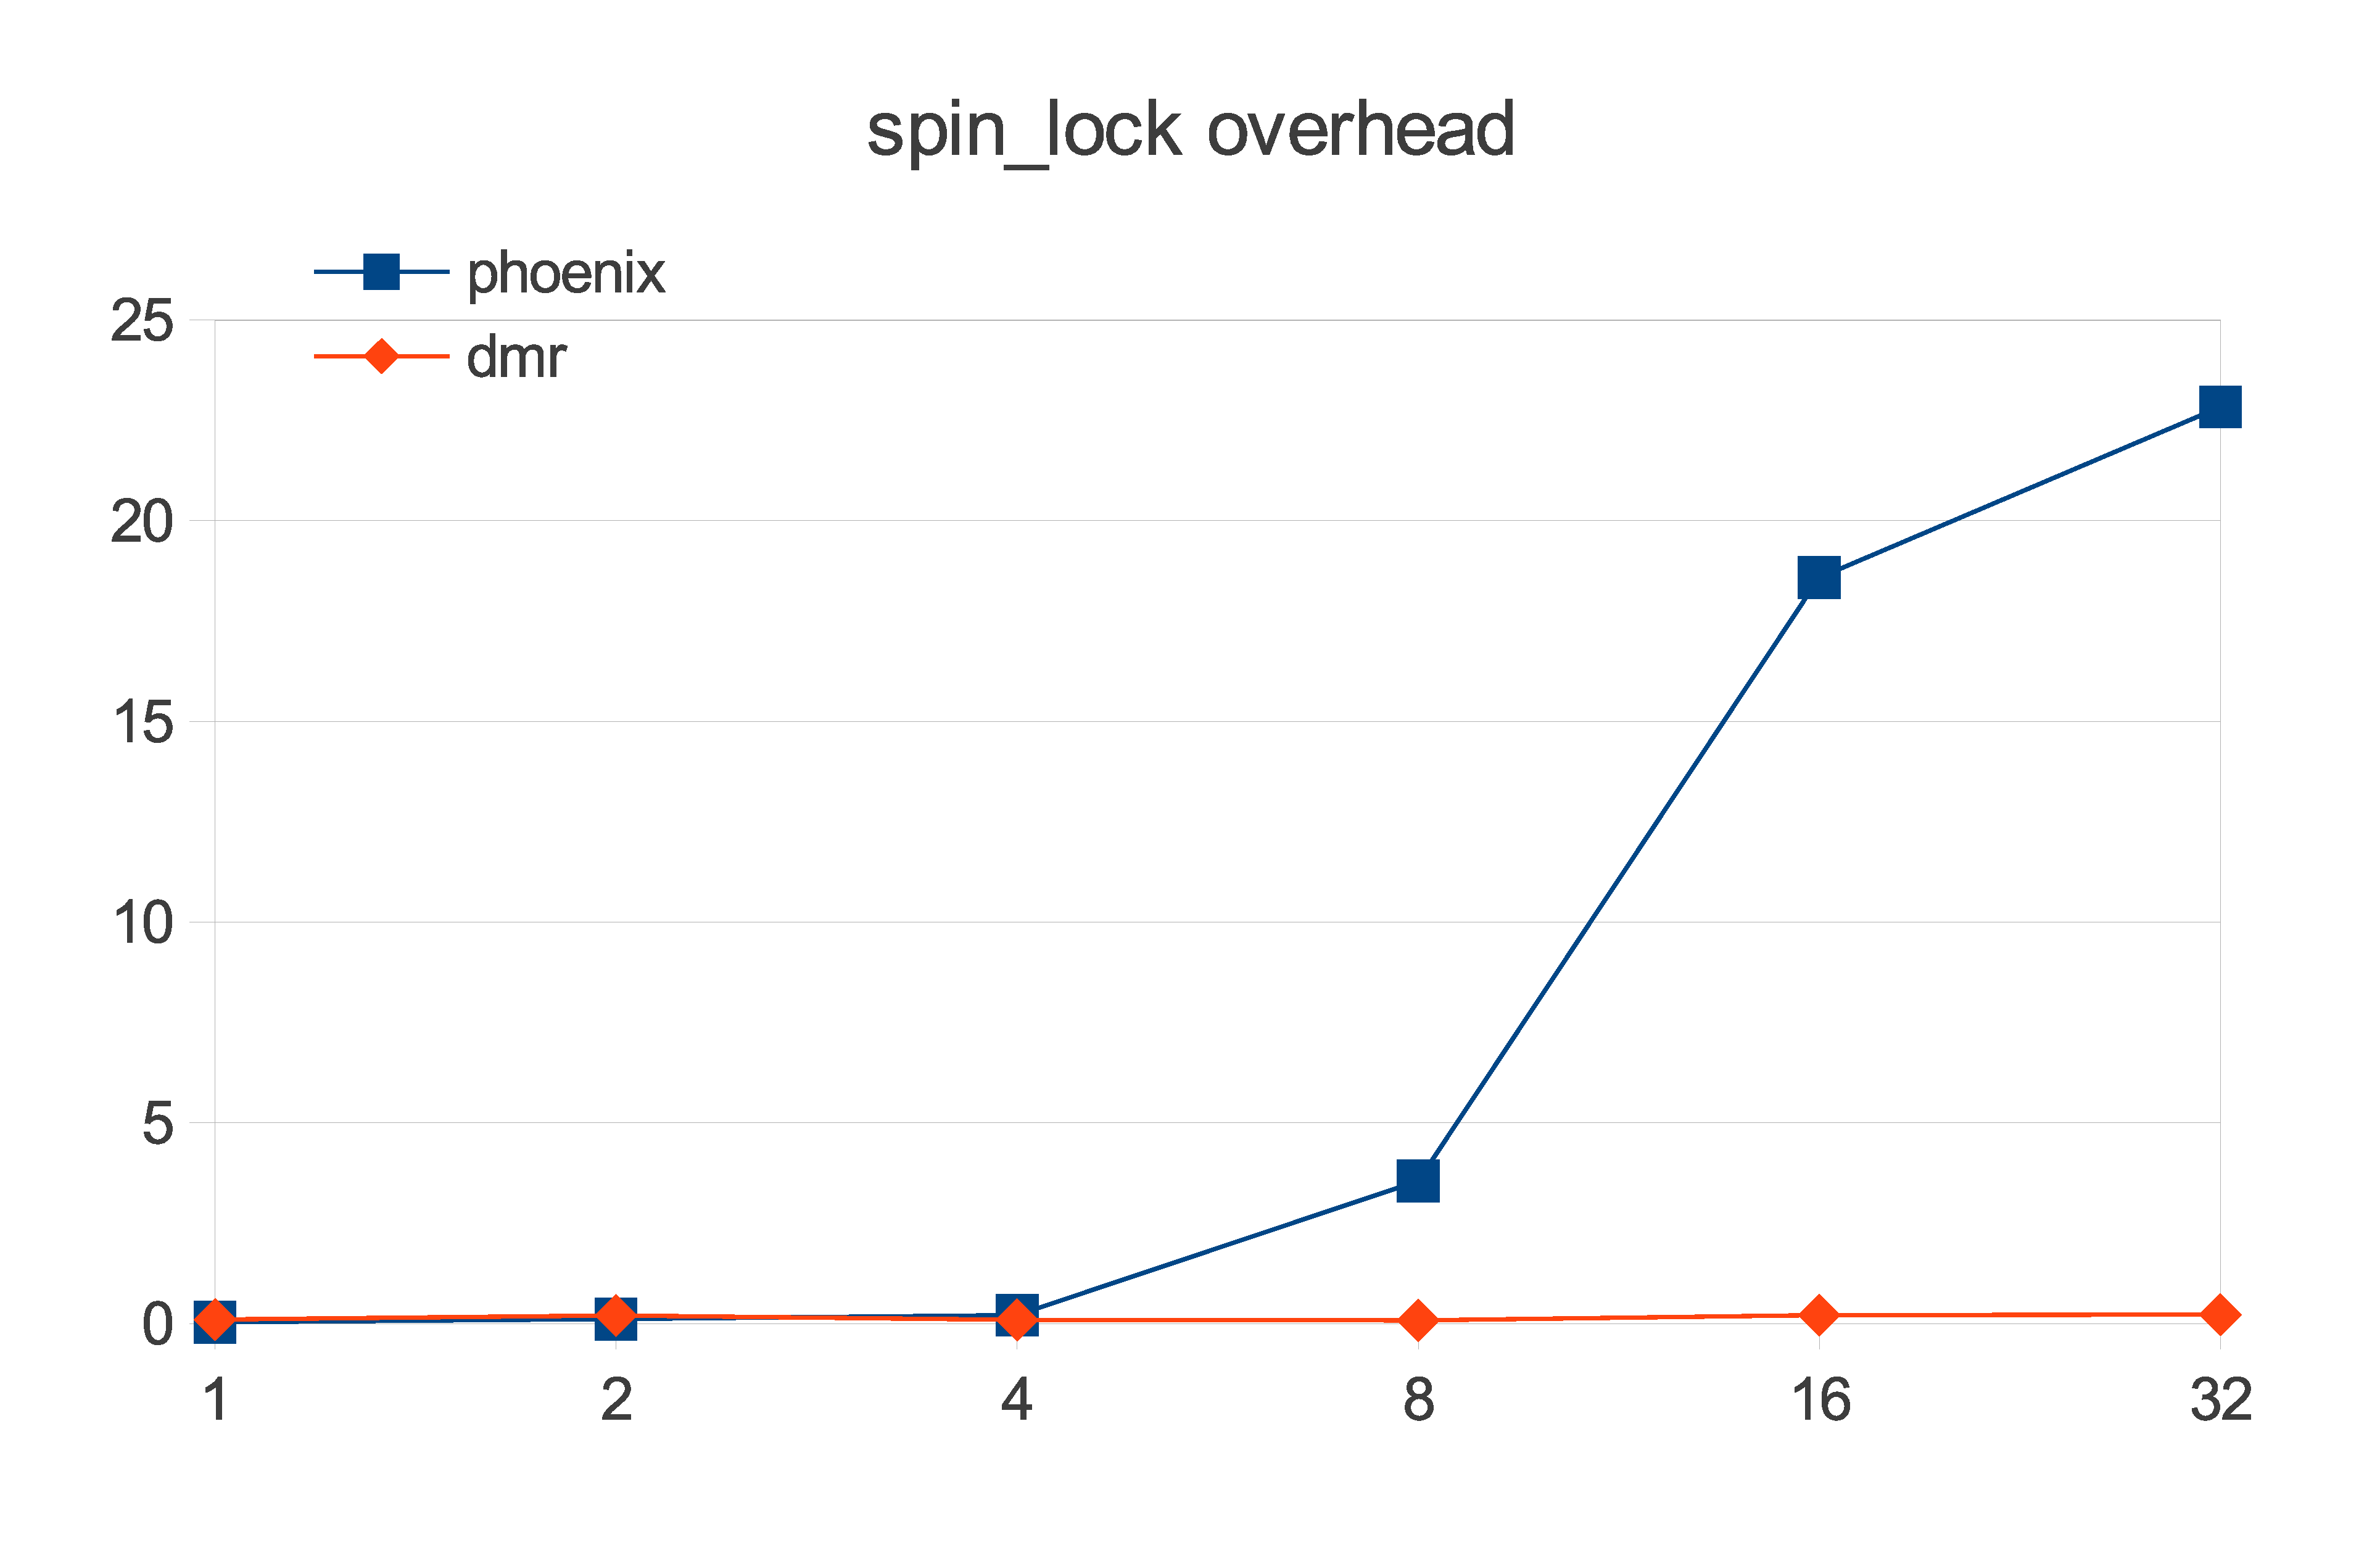
\includegraphics[width=0.45\textwidth]{eps/perf_spinlock.eps}
    \caption{spin lock overhead as core increasing}
    \label{fig:perf:spinlock}
\end{figure}

Figure \ref{fig:perf:utilized}
\begin{figure}[!h!t]  
    \centering
    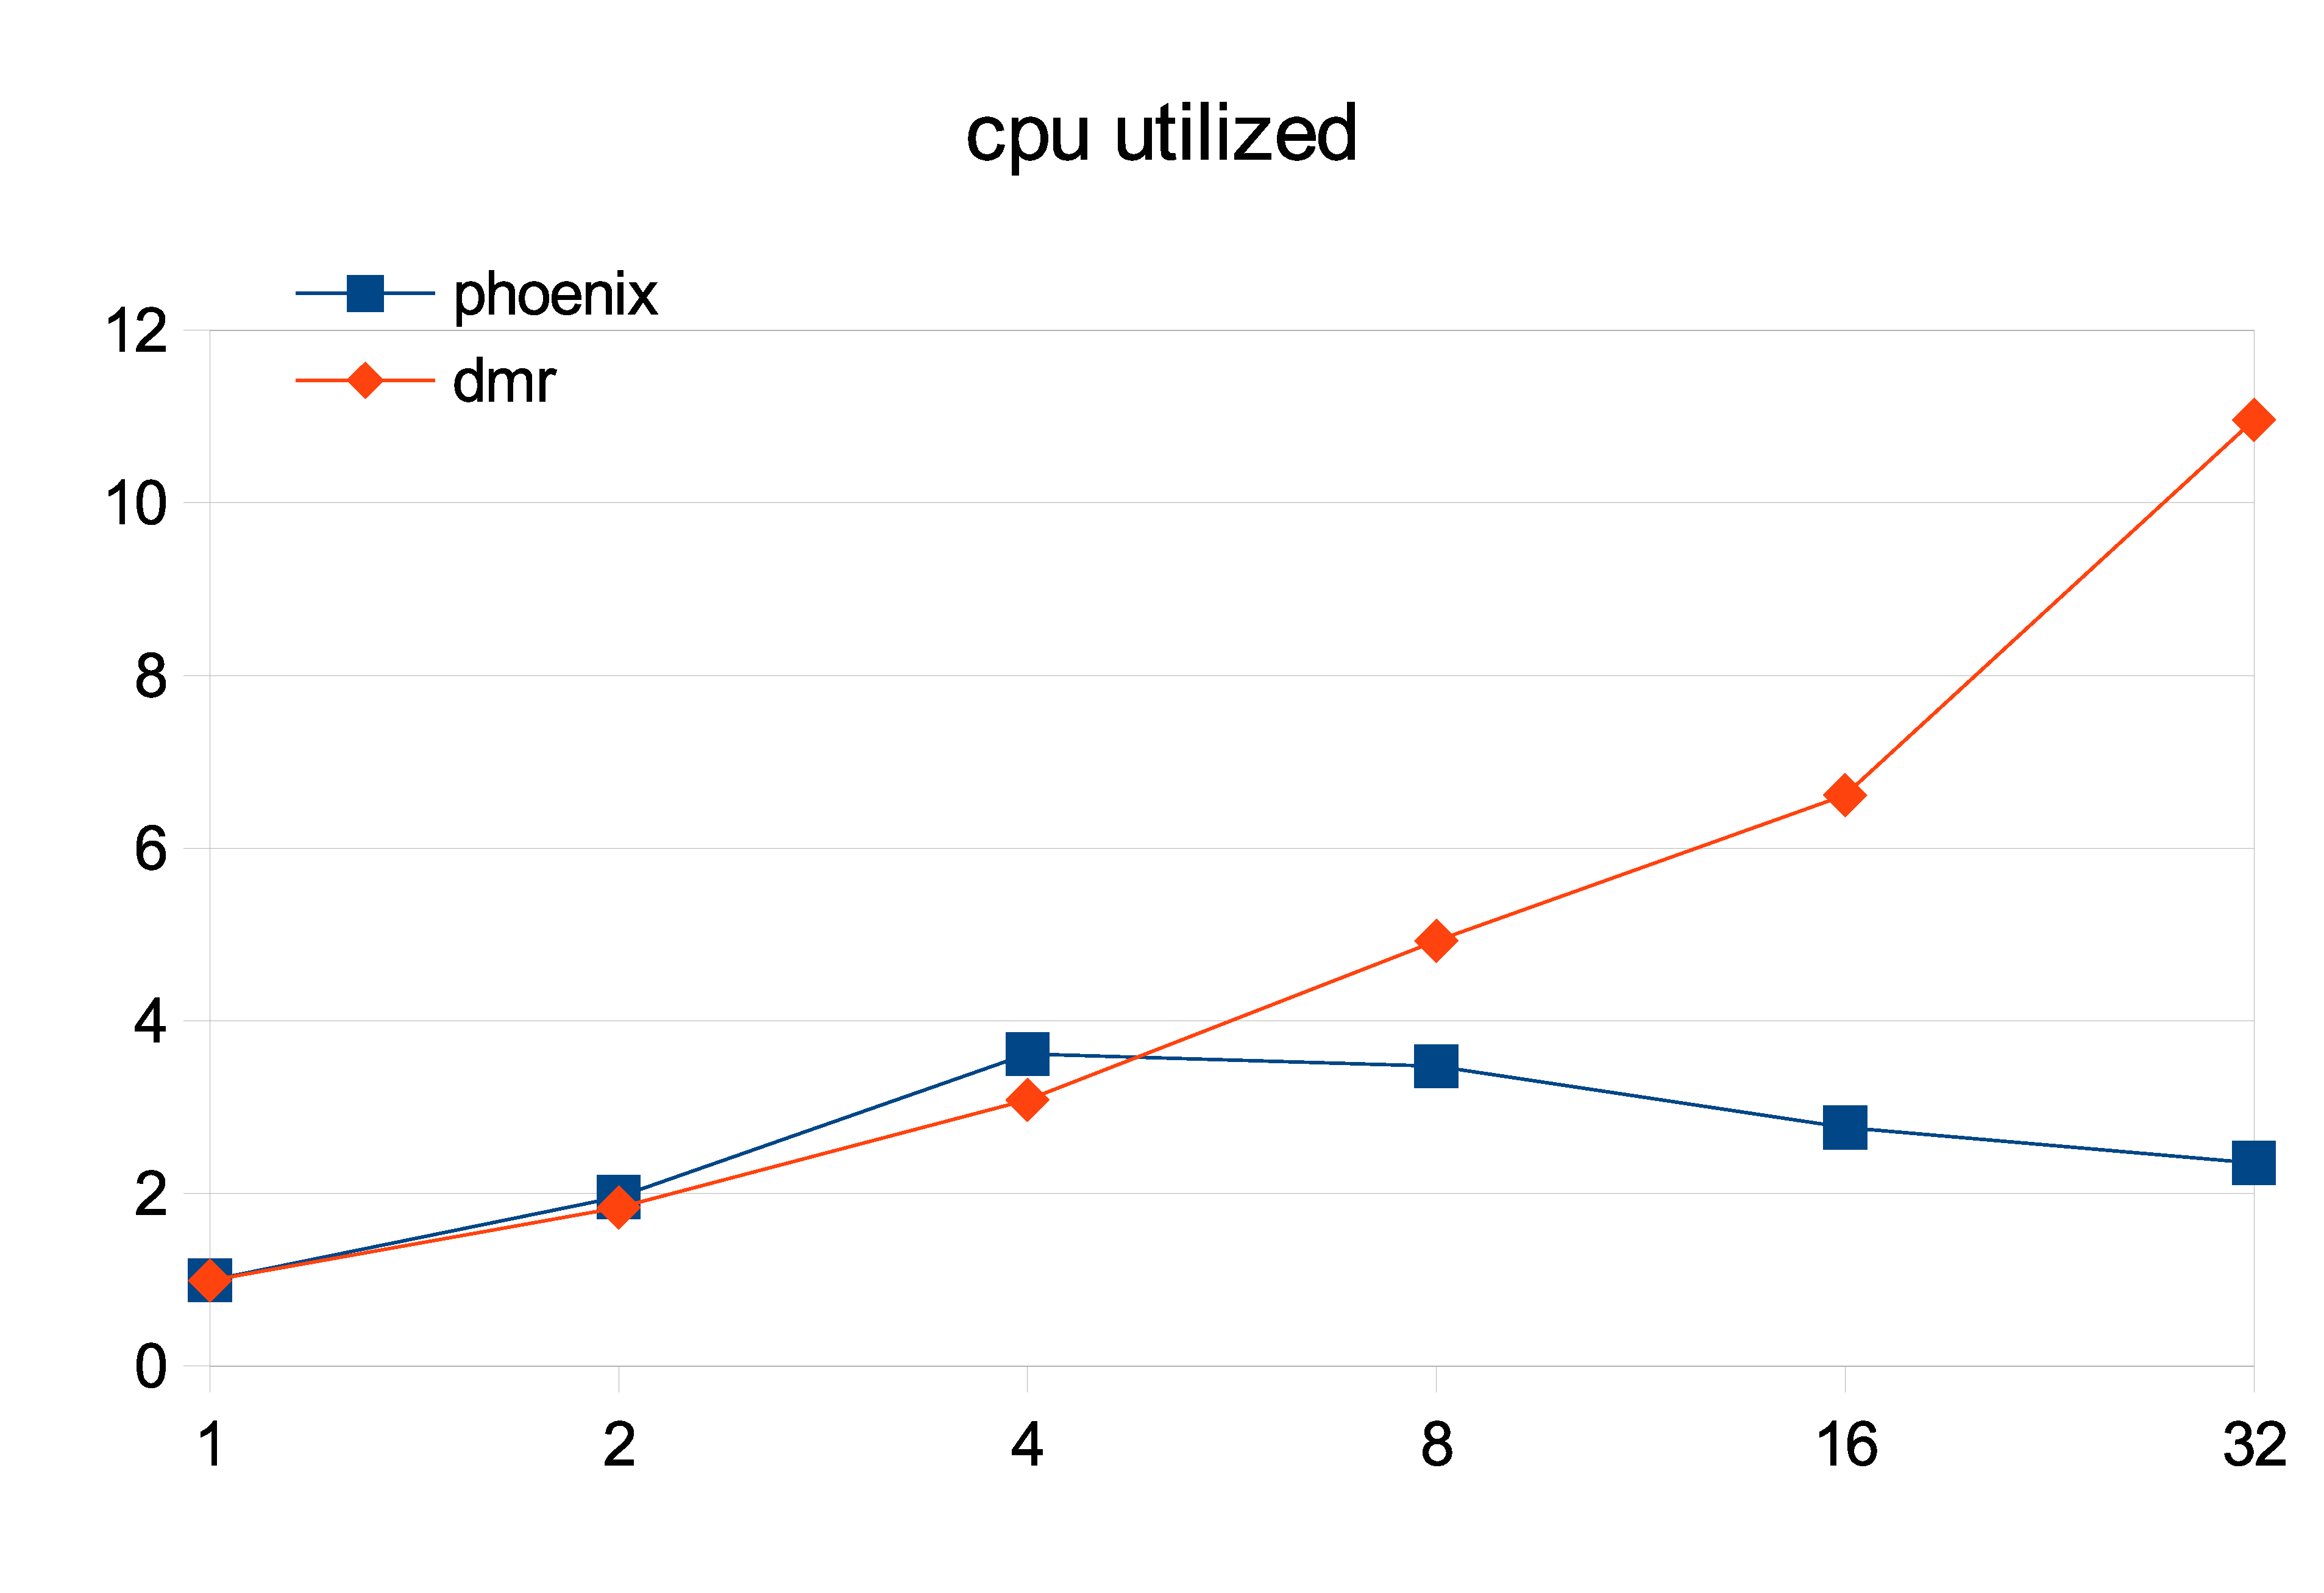
\includegraphics[width=0.45\textwidth]{eps/perf_utilized.eps}
    \caption{cpu utilized as core increasing}
    \label{fig:perf:utilized}
\end{figure}

System performance is evaluated using
instructions per cycle (IPC). Higher IPC means
better performance.
Figure \ref{fig:perf:ipc} shows the IPC of Phoenix first increases 
and then decreases as more threads are run on multi-core system.


\begin{figure}[!h!t]  
    \centering
    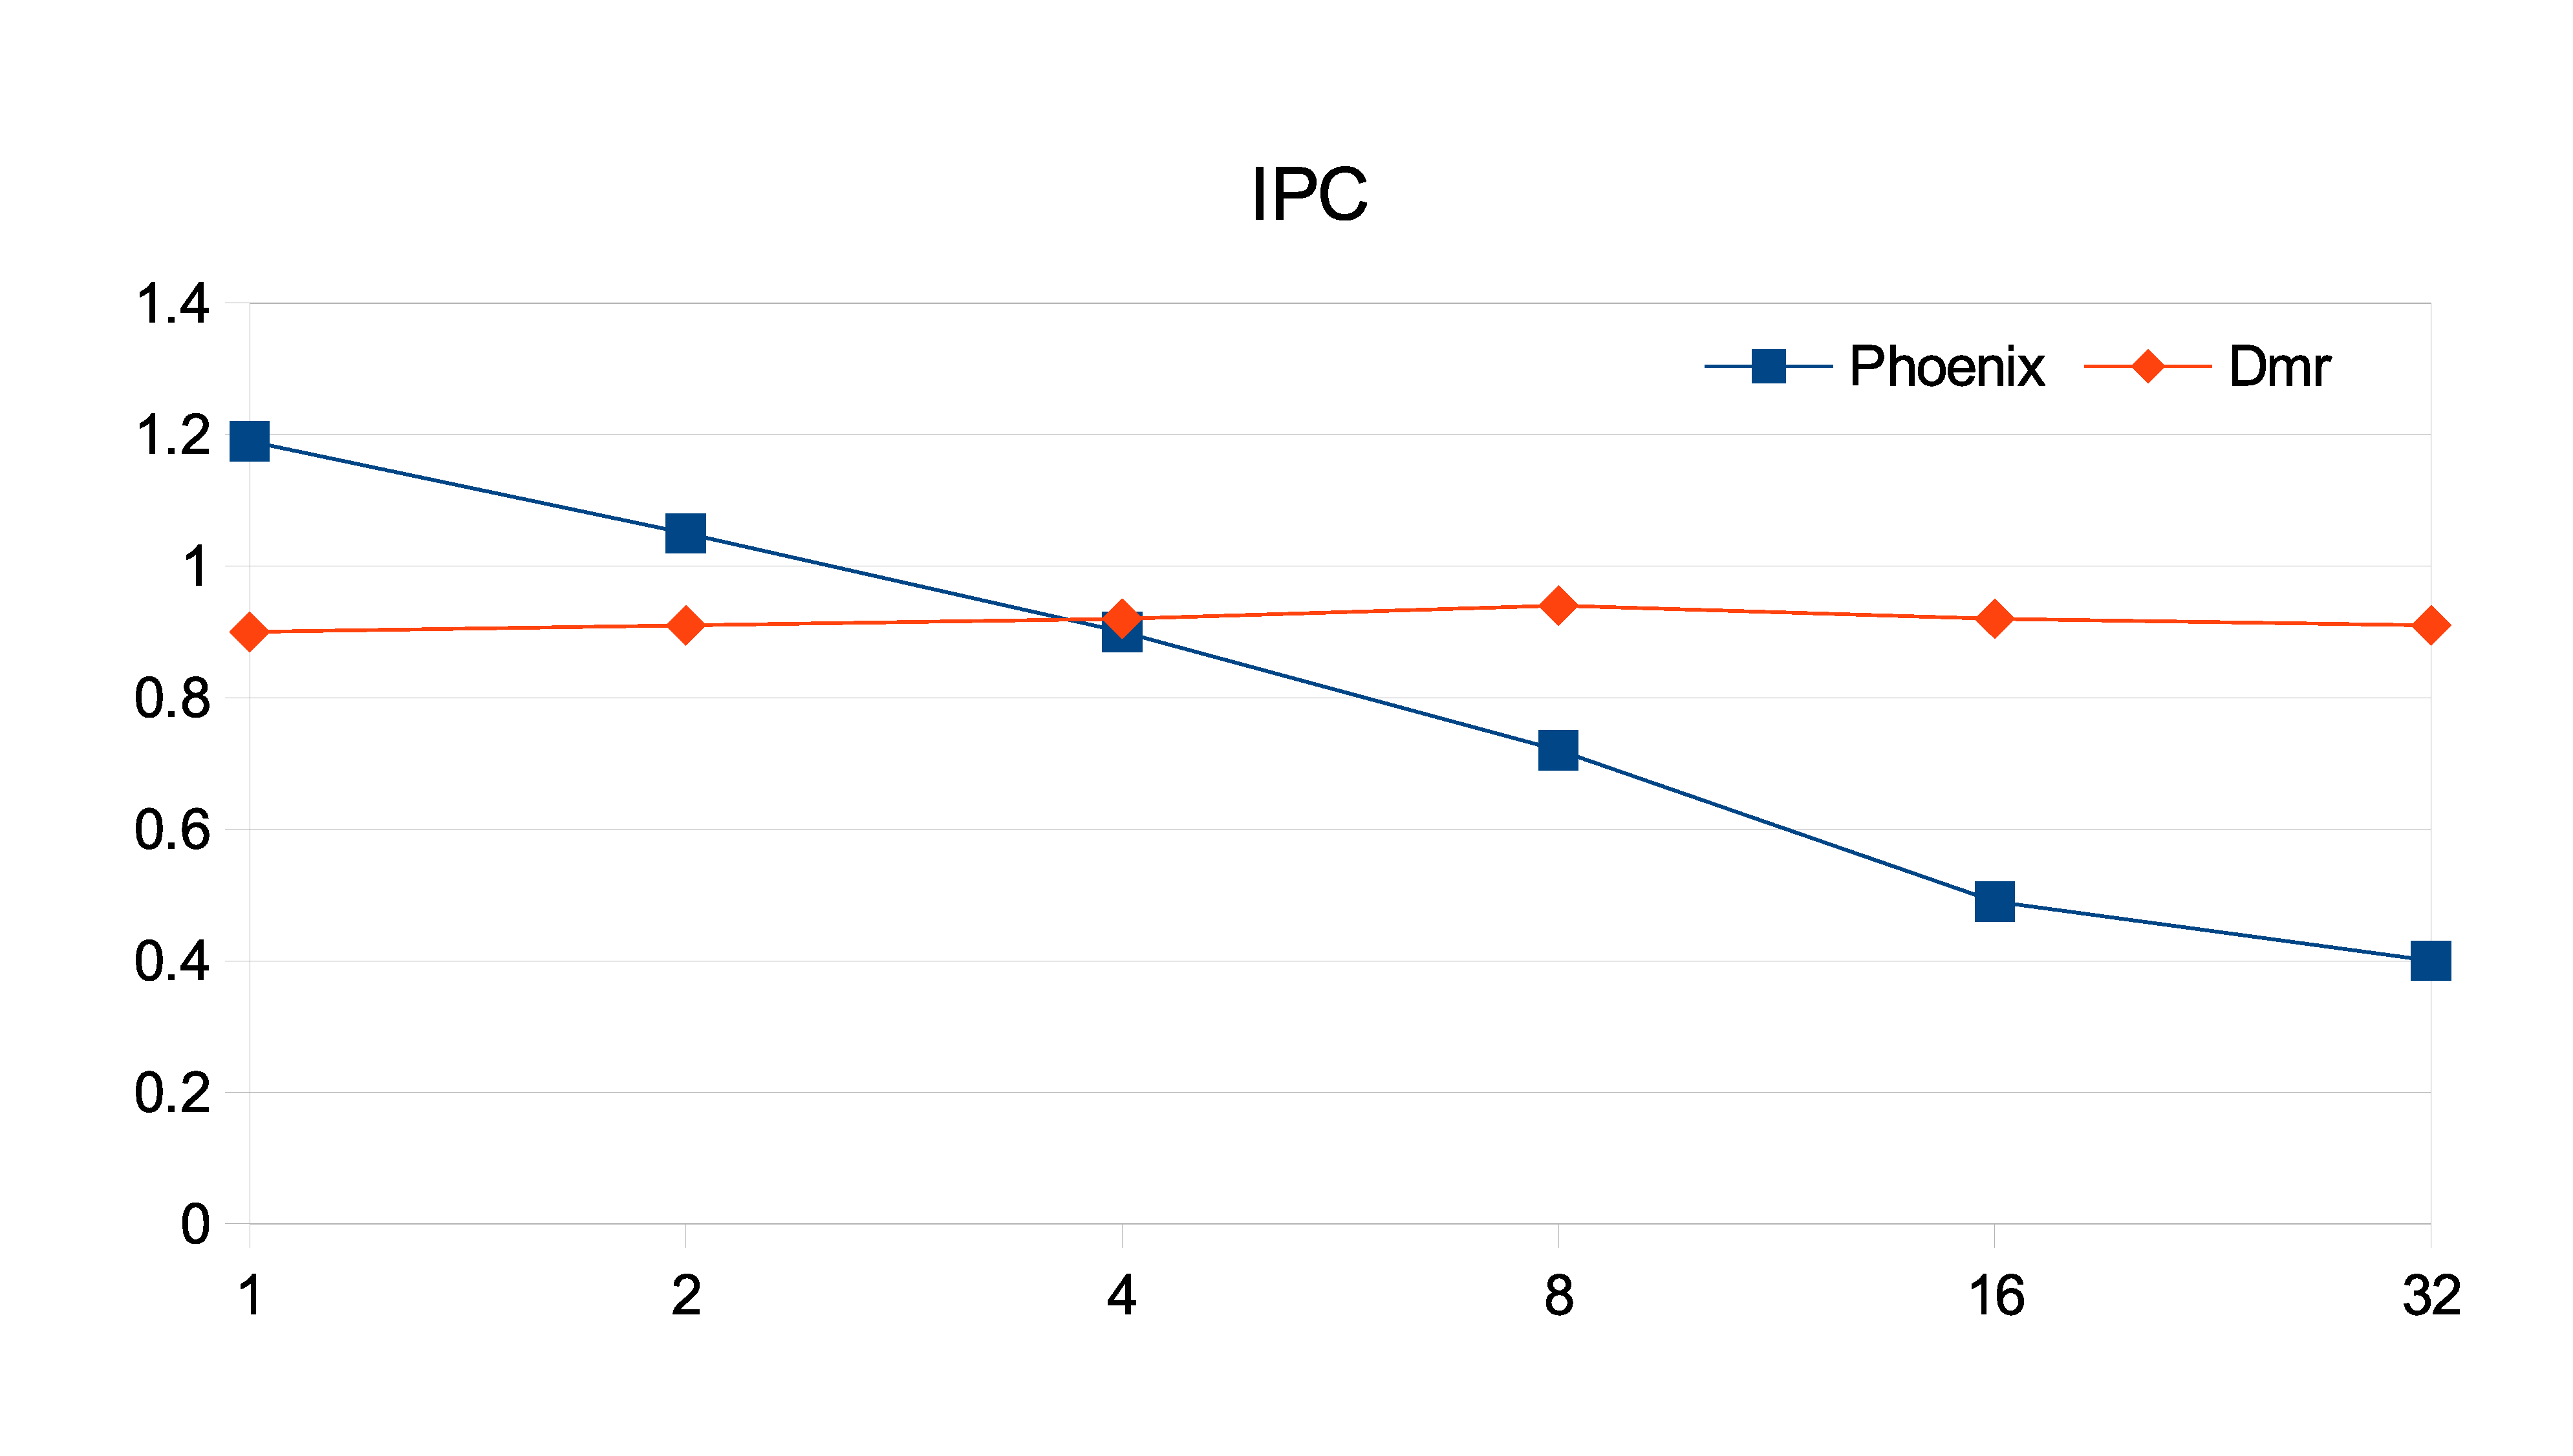
\includegraphics[width=0.45\textwidth]{eps/perf_ipc.eps}
    \caption{IPC}
    \label{fig:perf:ipc}
\end{figure}


\subsection{Tested Applications}


\subsection{Overall Performance}

\subsection{Fault Tolerance}
